\documentclass[11pt,a4paper]{article}

\usepackage[margin=1in]{geometry}
\usepackage{amsmath,amssymb}
\usepackage{booktabs}
\usepackage{graphicx}
\usepackage{microtype}
\usepackage{hyperref}

\hypersetup{
    colorlinks=true,
    linkcolor=blue!60!black,
    urlcolor=blue!60!black,
    citecolor=blue!60!black
}

\title{\textbf{Which Old Readings Matter?}\\
\large Local Geometry, Bottleneck Faces, and Zero-Net-Cost Steering in Aperiodic Surface Codes}
\author{K.~T.~Niedzwiecki\\
\small Independent Researcher, South Australia\\
\small \texttt{niedzkatie@gmail.com}}
\date{24 November 2026}

\begin{document}
\maketitle

\begin{abstract}
When a data qubit is lost on a surface-code patch, a decoder with access to past stabilizer readings outperforms an archive-free (``thin'', boundary-summary-only) decoder---especially when the lost edge sits on a shortest logical route. Here we ask a sharper follow-up question: \textbf{which specific archived readings actually carry that decoding advantage, how do neighboring faces back each other up, and why do endpoint omissions flip dozens of decisions while leaving the net score flat?} Using exhaustive zero-, one-, and two-fault evaluation ($385{,}648$ histories per site; bounded $(3,3)$ decoder, $p = 0.001$) across five $n=21$, distance-$(3,3)$ Ammann--Beenker (AB) and Penrose patches, we find five connected results:
\begin{itemize}
    \item \textbf{The ``Narrow Now'' holds across both tilings.} Once an indexing bug in the original adapter is corrected (11-check address audit), keeping just \textbf{eight} archived readings---two early rounds from the four stabilizer checks incident to the lost edge---recovers \textbf{97.25--99.26\%} of the full-archive accuracy gain across all five tested sites.
    \item \textbf{Hidden bottleneck faces.} Withholding just two archived readings from a single adjacent $Z$-face reveals a 16-fold split on \texttt{AB\_1 (e14)}: omitting face \texttt{Z3} collapses surviving gain to \textbf{15.54\%} ($+0.08425$~pp cost), whereas omitting its partner \texttt{Z6} retains \textbf{92.19\%} ($+0.00522$~pp cost)---a \textbf{16.14$\times$} cost ratio between two weight-4 $Z$-checks sharing the same lost edge. By contrast, at \texttt{Penrose\_1 (e14)}, either face alone preserved about \textbf{78\%} of the full-archive gain (\textbf{77.71\%} / \textbf{77.51\%}), whereas withholding both left just \textbf{0.083\%} (\texttt{Penrose\_2 (e4)} showed the same pattern: \textbf{81.12\%} / \textbf{80.82\%} alone vs.\ \textbf{0.025\%} with both withheld).
    \item \textbf{Local geometry drives the collapse across both tiling families ($2\times 2$ role reversal).} A complete census of all $1{,}220$ on-route eligible edges in the frozen $n=21$, $d=(3,3)$ AB and Penrose pools shows that \textbf{only two} local face-pair geometries occur in either family: \emph{Mirror Middle Yards} ($86.5\%$ in AB, $91.1\%$ in Penrose) and \emph{Hallway vs.\ Corner Ear} ($13.5\%$ in AB, $8.9\%$ in Penrose). In a pre-registered $2\times 2$ role reversal: (i)~enlarging \texttt{AB\_1} by \textbf{one extra tile} touching \texttt{Z6} (and re-cutting the boundary to keep $n=21$, $d=(3,3)$) yields \texttt{AB\_bal} on the exact same physical loss edge, lifting \texttt{Z3}'s surviving gain from \textbf{15.54\% $\to$ 72.59\%} and cutting the face cost ratio by more than $8\times$ (\textbf{16.14$\times$ $\to$ 1.96$\times$}); (ii)~selecting a Penrose cut with a degree-2 corner ear (\texttt{Penrose\_ear}) reproduces and sharpens the collapse: omitting hallway \texttt{Z7} crashes surviving gain to \textbf{14.23\%}, while omitting corner ear \texttt{Z6} retains \textbf{95.66\%} (\textbf{26.67$\times$} cost ratio).
    \item \textbf{Middle yards back each other up; corner ears cannot (5-site paired-face omission).} Covering \textbf{both} adjacent faces at once (retaining only the two endpoint $X$-checks) collapses surviving gain to \textbf{0.019--0.112\%} across all five sites. The substitution interaction $I$---how much extra it costs to lose one face once its partner is already gone---jumps $\sim 5$--$6\times$ with local shape across both tilings: \textbf{$I = +0.0455$ to $+0.0690$~pp} ($\sim 56$--$63\%$ of full gain) for all three middle-yard pairs (\texttt{Penrose\_1}, \texttt{Penrose\_2}, \texttt{AB\_bal}), versus just \textbf{$I = +0.0107$ to $+0.0109$~pp} ($\sim 10$--$11\%$) for both hallway-vs.-corner-ear pairs (\texttt{AB\_1}, \texttt{Penrose\_ear}).
    \item \textbf{Zero-net-cost decision steering comes from exact $X$-logical twinning.} On \texttt{Penrose\_2 (e4)}, withholding endpoint $X$-check \texttt{X5} (\texttt{X0}) yields \textbf{0.00000000~pp} net cost while flipping \textbf{44} (\textbf{18}) individual decoding decisions. Exhaustive flip-pairing analysis proves this zero is an exact structural symmetry: every single flipped history belongs to a same-record twin pair ($22/22$ on \texttt{X5}, $9/9$ on \texttt{X0}) whose total $X$-faults differ by the exact on-route weight-3 $X$-logical $\{4, 6, 10\}$---identical syndrome, identical decoder decision, opposite truth. On \texttt{Penrose\_1 (e14)}, the same $\{1, 10, 17\}$ twinning accounts for nearly all $570+$ flips, leaving $24$ unpaired movers that carry the tiny $+0.00001844$~pp residue.
\end{itemize}
\end{abstract}

\section{Introduction}
A fault-tolerant decoder with a finite memory budget faces a concrete version of a broader question: \emph{what from the past must be kept so that the present can still decide accurately?} In topological surface codes~\cite{Dennis2002}, qubit loss is a well-studied failure mode~\cite{Stace2009}, and recent delayed-loss decoders show that past stabilizer records can still be leveraged even when the exact round of loss is unknown~\cite{Baranes2026}. While aperiodic tilings have also been explored directly as quantum error-correcting codes~\cite{LiBoyle2023}, here Ammann--Beenker (AB) and Penrose tilings supply the planar cell-complex layouts for standard distance-$(3,3)$ surface-code patches. In a recent prospective study on fresh AB and Penrose patches (\texttt{AB\_1}, \texttt{Penrose\_1}, \texttt{Penrose\_2}), we confirmed that full-archive memory helps most when a lost edge lies on a shortest $X$-logical route---producing a $22$--$40\times$ brighter archive advantage on-route than at matched off-route edges.

At first glance, that study appeared to carry a puzzling second result: keeping only the eight local archived readings touching the lost edge (the ``diamond'' bracket) seemed to recover almost none of the on-route advantage. An independent address audit revealed why: on $11\times 9$ ($H_X \times H_Z$) patches, the legacy adapter had mapped $Z$-check indices assuming $10$ $X$-rows, silently querying the wrong checks. Once the address map was fixed, the picture flipped completely: \textbf{97.25--98.97\%} of the full-archive benefit lived right inside the four checks touching the lost edge.

That sharp localization opened three interlocking questions: if nearly the entire memory advantage lives inside four local checks (two adjacent $Z$-faces and two endpoint $X$-checks), \emph{(1) how is the load split between the two faces, (2) how much can one face stand in when the other is lost, and (3) why can omitting an endpoint flip dozens of decisions while leaving the net score untouched?} As the experiments below show, all three answers trace back to the same local object: the shortest weight-3 $X$-logical threading the lost edge and the boundary geometry immediately flanking it.

\section{Experimental Setup and Pre-Registered Lineage}
All experiments share the same pinned geometry generator, XOR syndrome simulator, shared-onset erasure inference, and bounded $(3,3)$ decoder ($w_{\mathrm{dec}} = 3$, $w_{\mathrm{frame}} = 3$, physical error rate $p = 0.001$), evaluated exhaustively over all zero-, one-, and two-fault ordinary configurations ($48{,}206$ configurations $\times$ $8$ onset/free-value variants = \textbf{385,648 histories per site}).

\begin{itemize}
    \item \textbf{Corrected local bracket (``intact''):} Retains rounds $t \in \{1, 2\}$ of the four checks geometrically incident to the lost edge (8 archived coordinates), plus live rounds $t \in \{3, 4\}$ of all checks, thin-state boundary parities, and the committed frame.
    \item \textbf{Single- and paired-witness omission:} Removes rounds $t \in \{1, 2\}$ of one named incident check (leaving 6 archived coordinates) or both adjacent $Z$-faces simultaneously (arm~$0$, leaving only the 4 early endpoint $X$-readings). Withheld coordinates are strictly \textbf{absent}, never zero-filled; live rounds, boundary parities, and frame remain untouched.
    \item \textbf{Primary score:} Weighted tie-aware truth credit (ties receive $0.5$ credit), reported in percentage points (pp). Omission cost is $100 \times (\text{intact credit} - \text{omission credit})$; positive cost means withholding hurt. Weighted credit \emph{lost} and \emph{gained} are tracked separately alongside unweighted label and tie-status flips.
    \item \textbf{Validation:} Every site completed deterministic unaccelerated full-scan verification samples with \textbf{0 mismatches} and $\max |\Delta p_0| = 0.0$, plus exact rational half-credit re-aggregation across all $1{,}928{,}240$ paired-face site-histories.
\end{itemize}

\section{Pillar 1 --- The ``Narrow Now'' Baseline}
Across the three original fresh cuts and the two new role-reversal cuts, retaining only the four local witnesses touching the lost edge captures nearly the entire full-archive gain (Table~\ref{tab:narrow} and Figure~\ref{fig:narrow}).

\begin{table}[h]
\centering
\caption{Local 8-reading (``intact'') recovery of full-archive gain across all five tested sites.}
\label{tab:narrow}
\begin{tabular}{llrrr}
\toprule
Site & Tiling & Full gain (pp) & Intact gain (pp) & Recovery (\% of full) \\
\midrule
\texttt{AB\_1 (e14)} & Ammann--Beenker & $+0.103101$ & $+0.100270$ & \textbf{97.25\%} \\
\texttt{Penrose\_1 (e14)} & Penrose & $+0.122290$ & $+0.120741$ & \textbf{98.73\%} \\
\texttt{Penrose\_2 (e4)} & Penrose & $+0.072349$ & $+0.071602$ & \textbf{98.97\%} \\
\texttt{AB\_bal (e14)} \textit{(new)} & Ammann--Beenker & $+0.096195$ & $+0.095485$ & \textbf{99.26\%} \\
\texttt{Penrose\_ear (e13)} \textit{(new)} & Penrose & $+0.099118$ & $+0.097956$ & \textbf{98.83\%} \\
\bottomrule
\end{tabular}
\end{table}

\begin{figure}[h]
\centering
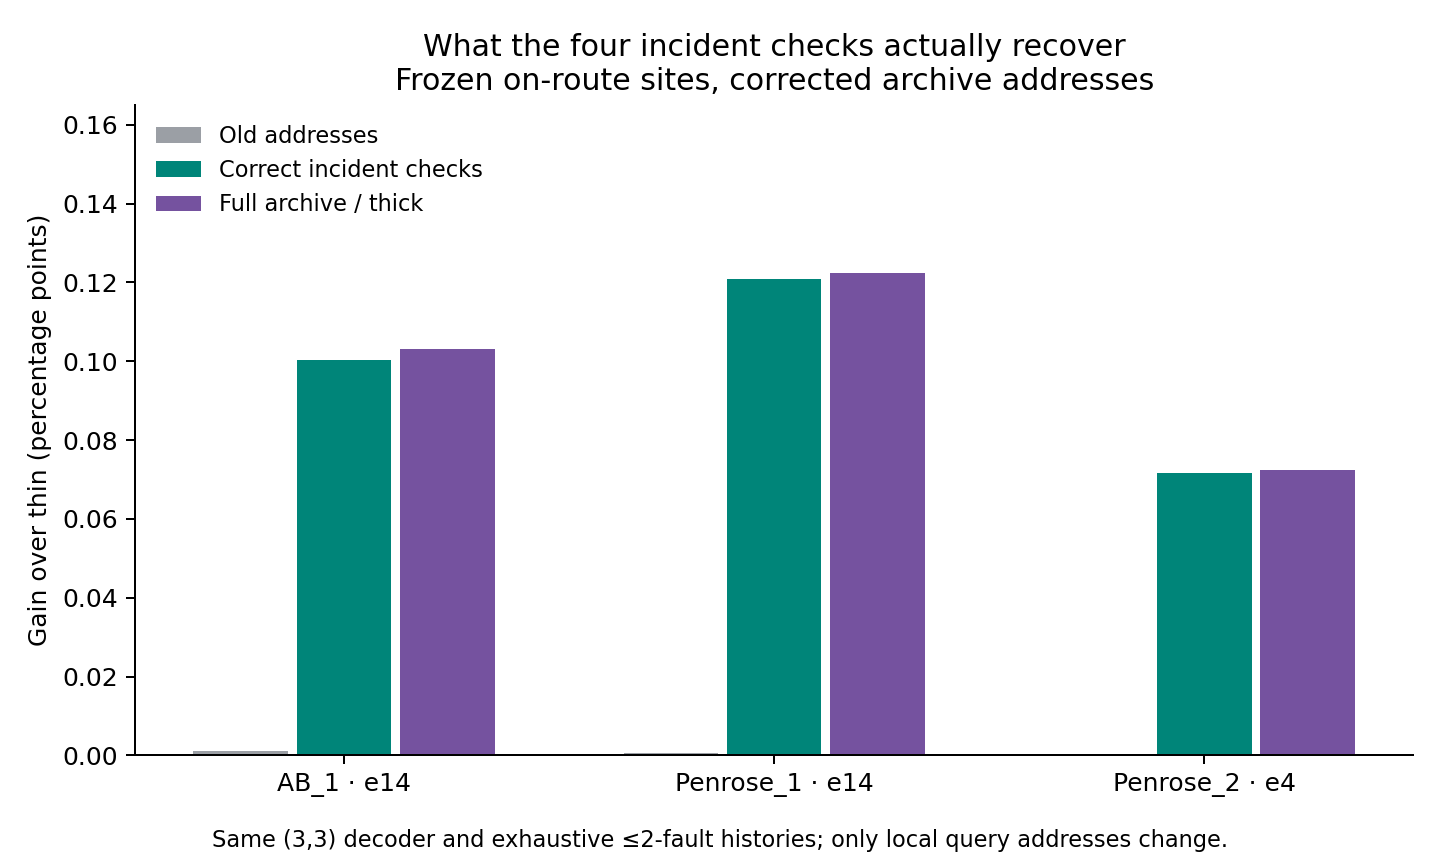
\includegraphics[width=0.92\linewidth]{figures/fig1_narrow_now_recovery.png}
\caption{Corrected local 8-reading recovery across the original fresh cuts (\texttt{audit/fresh-site-addresses-2026-11-20}).}
\label{fig:narrow}
\end{figure}

\section{Pillar 2 --- Single-Witness Omission and Paired-Face Backup}
\subsection{The 12-arm single-witness stress test}
Withholding one incident check at a time across the three original sites (Figure~\ref{fig:omission} and Table~\ref{tab:omission}) exposed a 16-fold asymmetry on \texttt{AB\_1} alongside balanced load-sharing on both Penrose patches. On \texttt{AB\_1}, \texttt{Z3} and \texttt{Z6} are both weight-4 $Z$-checks sitting on opposite sides of the exact same lost edge \texttt{e14}, yet omitting \texttt{Z3} costs \textbf{16.14$\times$} more than omitting \texttt{Z6}.

\begin{table}[h]
\centering
\caption{Twelve-arm witness-omission results across \texttt{AB\_1}, \texttt{Penrose\_1}, and \texttt{Penrose\_2}.}
\label{tab:omission}
\begin{tabular}{lllrrrr}
\toprule
Site & Omitted & Role / wt & Cost (pp) & Surviving (\% full) & Label flips & Tie flips \\
\midrule
\texttt{AB\_1 (e14)} & \texttt{X4} / \texttt{X5} & endpoint / 5 & $+0.000184$ & 97.08\% & 82 / 90 & 8 / 8 \\
\texttt{AB\_1 (e14)} & \textbf{\texttt{Z3}} & \textbf{face / 4} & $\mathbf{+0.084253}$ & \textbf{15.54\%} & \textbf{4,785} & 4 \\
\texttt{AB\_1 (e14)} & \texttt{Z6} & face / 4 & $+0.005219$ & \textbf{92.19\%} & 2,112 & 4 \\
\texttt{Penrose\_1 (e14)} & \texttt{X4} / \texttt{X6} & endpoint / 6, 3 & $+0.000018$ & 98.72\% & 570 / 572 & 12 / 12 \\
\texttt{Penrose\_1 (e14)} & \texttt{Z1} & face / 4 & $+0.025708$ & \textbf{77.71\%} & 2,152 & 4 \\
\texttt{Penrose\_1 (e14)} & \texttt{Z7} & face / 4 & $+0.025948$ & \textbf{77.51\%} & 3,468 & 12 \\
\texttt{Penrose\_2 (e4)} & \texttt{X0} / \texttt{X5} & endpoint / 5, 3 & $\mathbf{0.000000}$ & 98.97\% & \textbf{18 / 44} & 2 / 2 \\
\texttt{Penrose\_2 (e4)} & \texttt{Z1} & face / 4 & $+0.013131$ & \textbf{80.82\%} & 1,368 & 14 \\
\texttt{Penrose\_2 (e4)} & \texttt{Z4} & face / 4 & $+0.012910$ & \textbf{81.12\%} & 2,480 & 10 \\
\bottomrule
\end{tabular}
\end{table}

\begin{figure}[h]
\centering
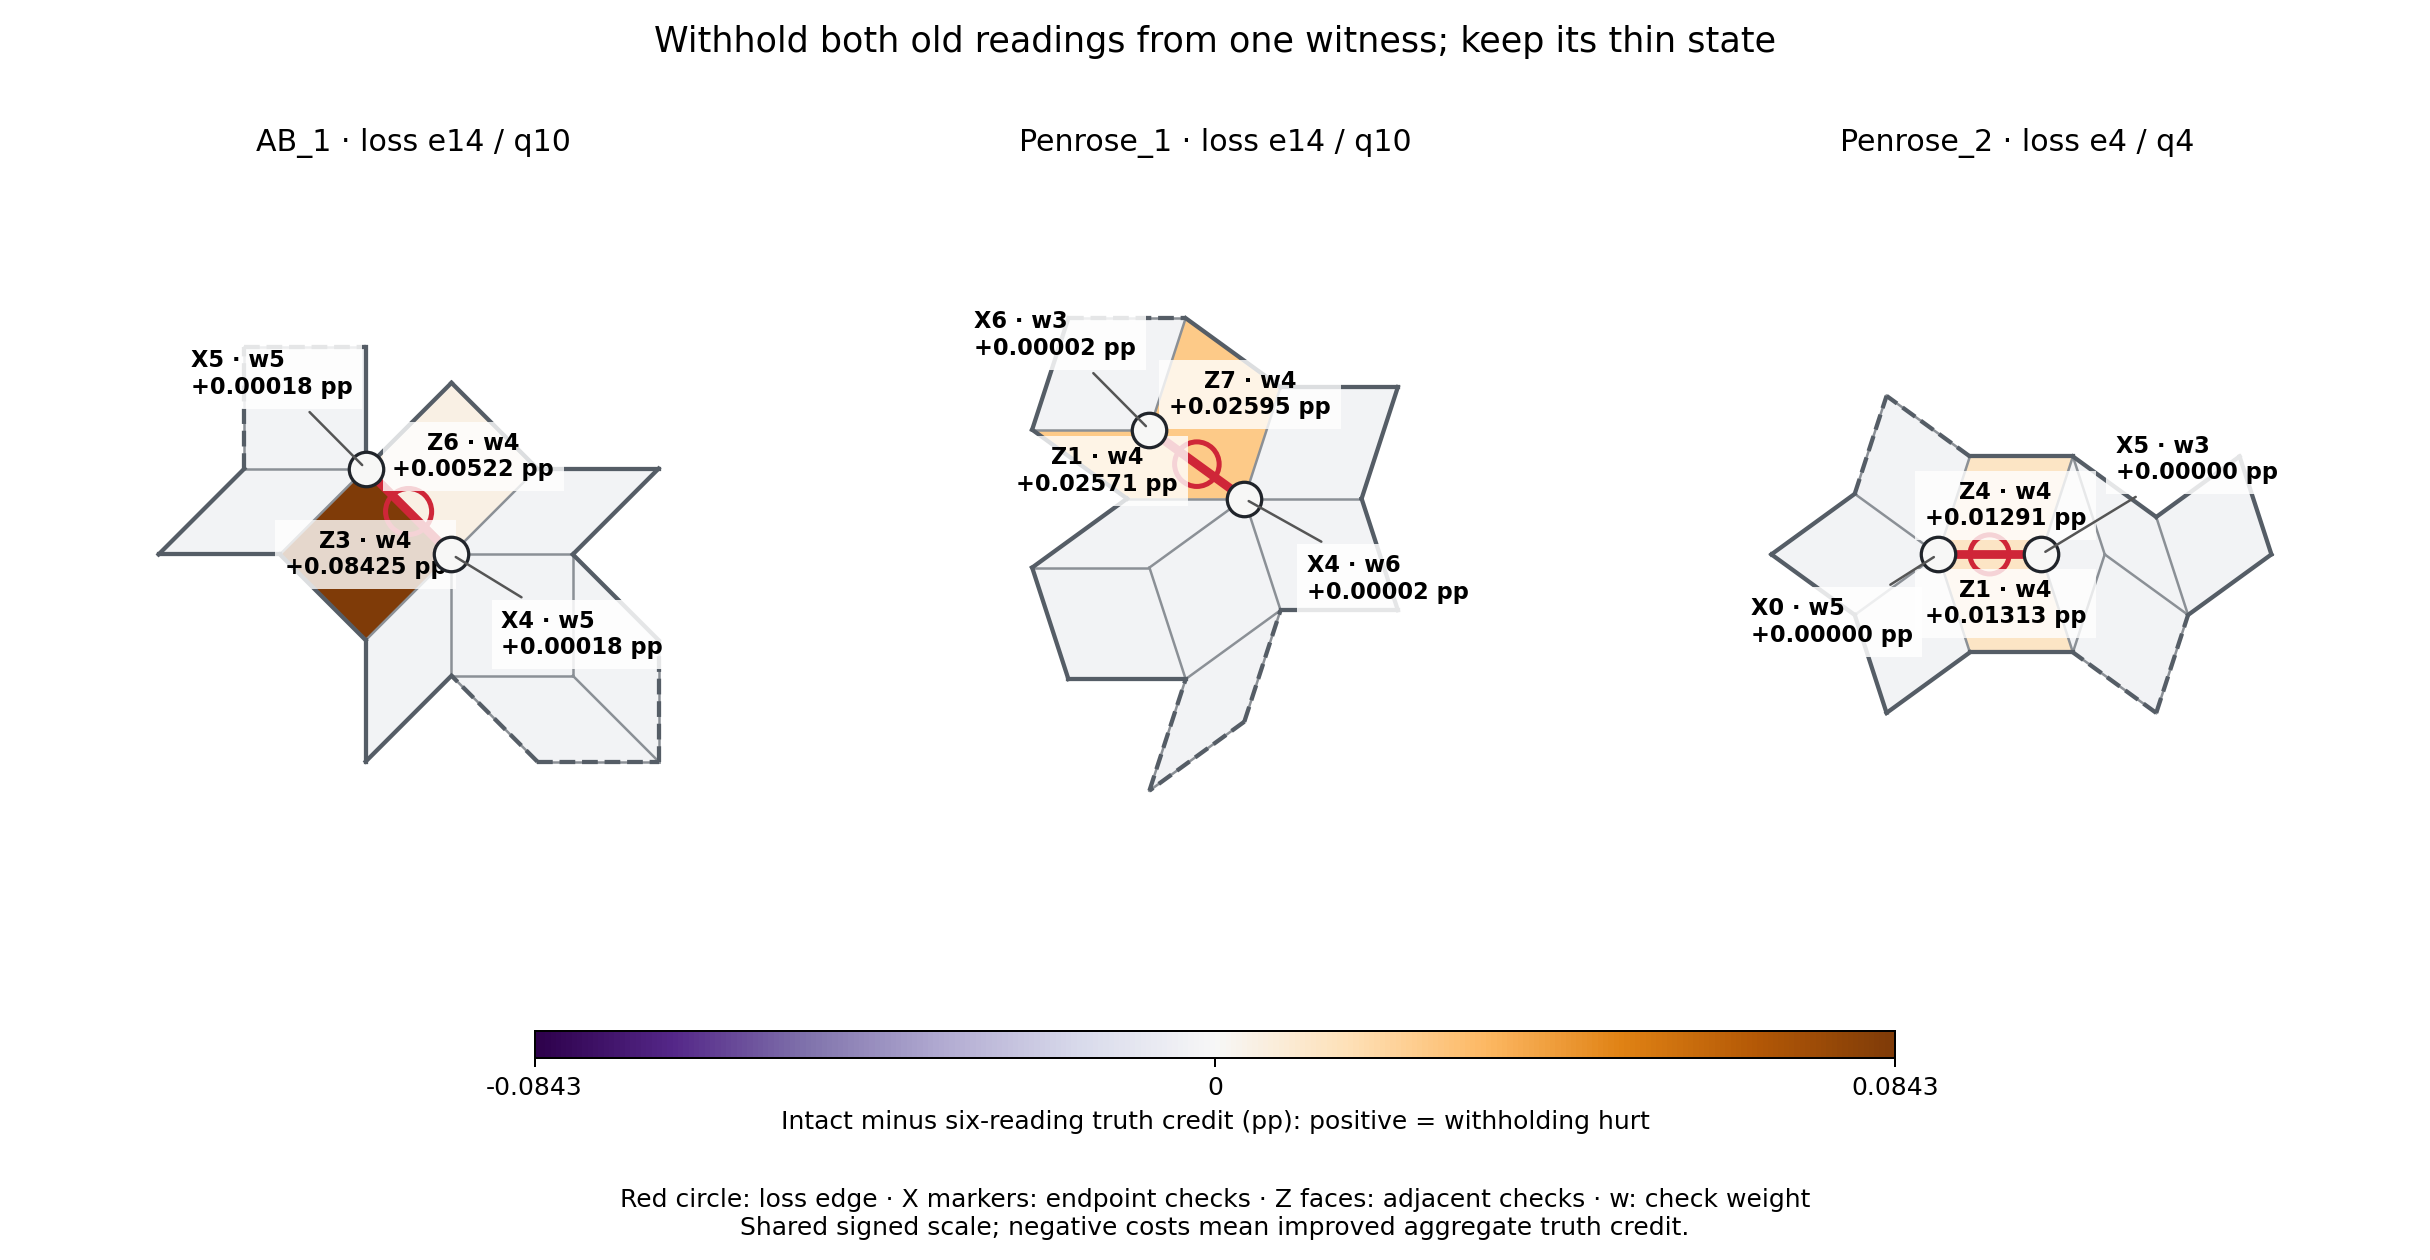
\includegraphics[width=0.95\linewidth]{figures/fig2_witness_omission_costs.png}
\caption{Three-panel omission cost map across \texttt{AB\_1}, \texttt{Penrose\_1}, and \texttt{Penrose\_2} (\texttt{experiment/local-witness-omission-2026-11-20}).}
\label{fig:omission}
\end{figure}

\subsection{Covering both faces: mutual backup vs.\ single-face bottlenecks}
A natural follow-up asks what survives when \textbf{both} adjacent $Z$-faces are covered simultaneously, leaving only the two endpoint $X$-checks (\texttt{experiment/paired-face-omission-2026-11-23}). Let $G_{AB}, G_A, G_B, G_0$ be the gains (over \texttt{thin}) when keeping both faces, $A$ only, $B$ only, or neither face, and let $I = (G_A - G_0) - (G_{AB} - G_B) = (G_B - G_0) - (G_{AB} - G_A)$ measure how much extra it costs to lose a face once its partner is already absent (Table~\ref{tab:paired} and Figure~\ref{fig:paired}).

\begin{table}[h]
\centering
\caption{Five-site paired-face retention arms and substitution interaction $I$ (\texttt{9515df3}).}
\label{tab:paired}
\begin{tabular}{llrrrrrr}
\toprule
Site ($A$ / $B$) & Shape & Both & $A$ only & $B$ only & Neither $G_0$ & $I$ (pp) & $I$/Full \\
\midrule
\texttt{AB\_1} (\texttt{Z3}/\texttt{Z6}) & Hallway / Ear & 97.25\% & 92.19\% & 15.54\% & \textbf{0.107\%} & $+0.01069$ & \textbf{10.4\%} \\
\texttt{Penrose\_ear} (\texttt{Z7}/\texttt{Z6}) & Hallway / Ear & 98.83\% & 95.66\% & 14.23\% & \textbf{0.112\%} & $+0.01085$ & \textbf{10.9\%} \\
\texttt{AB\_bal} (\texttt{Z3}/\texttt{Z6}) & Middle yards & 99.26\% & 85.69\% & 72.59\% & \textbf{0.019\%} & $+0.05676$ & \textbf{59.0\%} \\
\texttt{Penrose\_1} (\texttt{Z7}/\texttt{Z1}) & Middle yards & 98.73\% & 77.71\% & 77.51\% & \textbf{0.083\%} & $+0.06898$ & \textbf{56.4\%} \\
\texttt{Penrose\_2} (\texttt{Z1}/\texttt{Z4}) & Middle yards & 98.97\% & 81.12\% & 80.82\% & \textbf{0.025\%} & $+0.04554$ & \textbf{62.9\%} \\
\bottomrule
\end{tabular}
\end{table}

\begin{figure}[h]
\centering
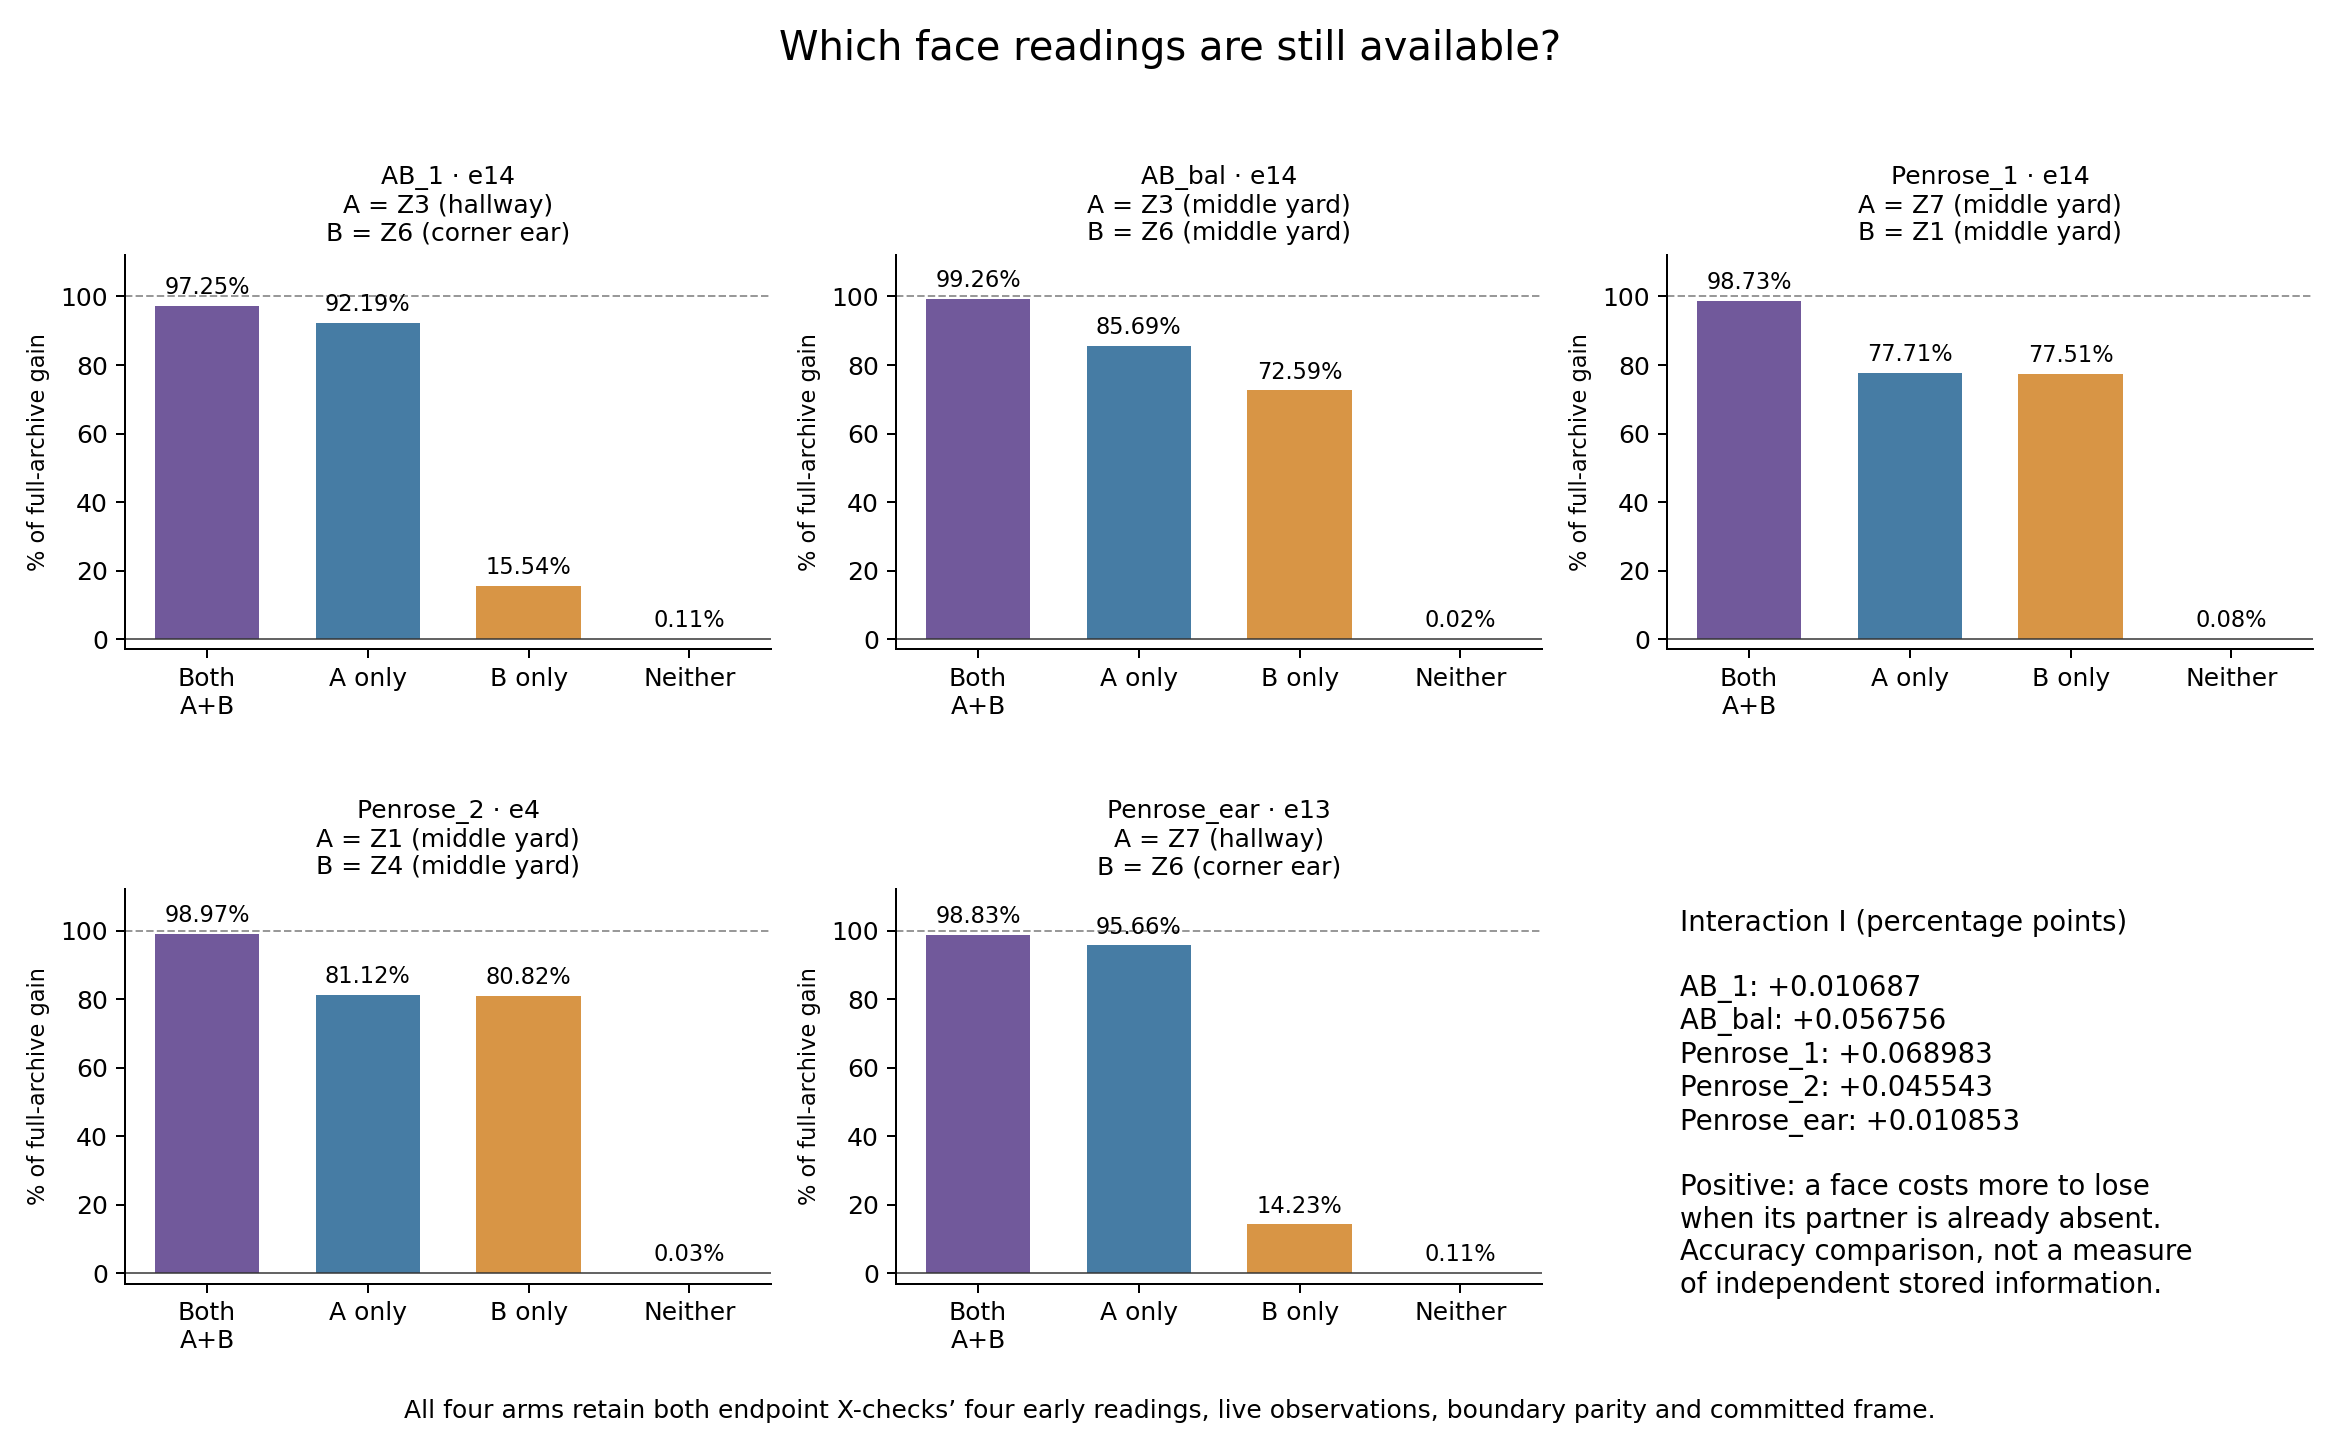
\includegraphics[width=0.95\linewidth]{figures/fig4_paired_face_backup.png}
\caption{Four-arm paired-face retention comparison across all five sites (\texttt{experiment/paired-face-omission-2026-11-23}).}
\label{fig:paired}
\end{figure}

Across all five sites, covering both faces wipes out $>99.88\%$ of local recovery ($0.019$--$0.112\%$ surviving). Yet the interaction $I$ cleanly splits the five sites into two regimes: when both neighbors are middle yards (\texttt{Penrose\_1}, \texttt{Penrose\_2}, \texttt{AB\_bal}), either face can stand in for \textbf{56--63\%} of the full-archive gain while its partner is absent; when one neighbor is a corner ear (\texttt{AB\_1}, \texttt{Penrose\_ear}), mutual backup collapses by $\sim 5$--$6\times$ to just \textbf{10--11\%}.

\section{Pillar 3 --- Local Bottleneck vs.\ Corner Ear and the $2\times 2$ Role Reversal}
\subsection{Structural diagnosis and complete pool census}
Read-only graph inspection of the sealed patch definitions explains the \texttt{AB\_1} split geometrically:
\begin{itemize}
    \item On \texttt{AB\_1 (e14)}, \texttt{Z3} ($\{5, 6, 7, 10\}$) is an \textbf{interior bridge (``hallway'')} with $1$ smooth boundary edge (\texttt{q5}), $3$ interior edges, $3$ neighboring $Z$-faces (\texttt{Z0, Z2, Z6}), and corner degrees $(3, 3, 5, 5)$. Both shortest (weight-3) $X$-logicals through \texttt{e14} ($\{5, 10, 14\}$ and $\{5, 10, 15\}$) funnel through \texttt{q5}. By contrast, \texttt{Z6} ($\{10, 11, 14, 15\}$) is a \textbf{protruding corner ear} with $2$ exposed smooth boundary edges (\texttt{q14, q15}) meeting at a \textbf{degree-2 corner tip} (\texttt{v12}, weight-2 check $\texttt{X7} = \{14, 15\}$), only $2$ interior edges, and only $2$ neighboring $Z$-faces (\texttt{Z3, Z7}). The two shortest $X$-logicals fork across \texttt{q14} vs.\ \texttt{q15} modulo \texttt{X7}.
    \item On \texttt{Penrose\_1} (\texttt{Z7} vs.\ \texttt{Z1}) and \texttt{Penrose\_2} (\texttt{Z1} vs.\ \texttt{Z4}), every face in both pairs is a \textbf{middle yard}: $1$ smooth boundary edge, $3$ interior edges, $3$ neighboring $Z$-faces, identical sorted corner degrees ($(3, 3, 3, 6)$ and $(3, 3, 4, 5)$), and a single symmetric $X$-logical exit.
\end{itemize}

Enumerating all on-route eligible edges in the frozen $n=21$, $d=(3,3)$ disk-cut generator shows that \textbf{only these two} local face-pair geometries occur in either tiling family: in AB ($1{,}282$ cuts, $503$ on-route edges), $435$ ($86.5\%$) are Mirror Middle Yards and $68$ ($13.5\%$) are Hallway + Corner Ear; in Penrose ($1{,}791$ cuts, $717$ on-route edges), $653$ ($91.1\%$) are Mirror Middle Yards and $64$ ($8.9\%$) are Hallway + Corner Ear.

\subsection{Pre-registered $2\times 2$ role reversal}
To separate local geometry from tiling family, we selected two role-reversal cuts from the frozen pool \emph{before} running the decoder:
\begin{enumerate}
    \item \texttt{AB\_bal} (\texttt{spec=(22, 2, 2, 10)}, \texttt{corners=(2, 5, 11, 15)}, \texttt{e14}): \texttt{AB\_1} enlarged by \textbf{one extra tile} (new \texttt{Z8}, sharing an edge with \texttt{Z6} and meeting \texttt{Z3} at a vertex) together with the boundary re-cut needed to maintain $n=21$, $d=(3,3)$ (four boundary edges swap rough/smooth assignment, two become interior, check split shifts $11\,X / 9\,Z \to 10\,X / 10\,Z$, and the scored $Z$ representative shifts physically). The physical loss-edge endpoints $(0,1,2,-1)$ and $(0,1,2,0)$ are identical (\texttt{q10} $\to$ \texttt{q9}), one of the two shortest $X$-logicals through the loss disappears while the other survives physically, and \texttt{Z3} and \texttt{Z6} become locally matched middle yards (corner degrees $(3,3,5,5)$).
    \item \texttt{Penrose\_ear} (\texttt{spec=(7, 1, 3, 10)}, \texttt{corners=(0, 4, 9, 13)}, \texttt{e13}): exact structural twin of \texttt{AB\_1}, pairing hallway \texttt{Z7} ($1$ smooth boundary edge, $3$ $Z$-neighbors) with protruding degree-2 corner ear \texttt{Z6} ($2$ smooth boundary edges, $2$ $Z$-neighbors, forked exits).
\end{enumerate}

Both predictions held cleanly (Table~\ref{tab:2x2} and Figure~\ref{fig:2x2}): giving Penrose a corner ear triggers an even sharper \textbf{26.67$\times$} collapse (\texttt{Z7} $\to 14.23\%$ vs.\ \texttt{Z6} $\to 95.66\%$), while enlarging \texttt{AB\_1} by one tile to fill in \texttt{Z6}'s corner ear eliminates the collapse (\texttt{Z3} jumps $15.54\% \to 72.59\%$, cost ratio drops $8\times$ from $16.14\times$ to $1.96\times$, and mutual backup $I$ jumps from $10.4\%$ to $59.0\%$).

\begin{table}[h]
\centering
\caption{Measured $2\times 2$ role-reversal matrix across all five sites (surviving \% of full-archive gain, face-cost ratio, and mutual backup $I$/Full).}
\label{tab:2x2}
\begin{tabular}{lll}
\toprule
Local shape around loss edge & Ammann--Beenker & Penrose \\
\midrule
\textbf{Two Middle Yards} & \texttt{AB\_bal (e14)} \textit{[new]}: & \texttt{Penrose\_1 (e14)}: 77.51\% vs.\ 77.71\% (1.01$\times$, $I{=}56.4\%$) \\
\textit{(1 bnd edge, 3 $Z$-nbrs each)} & \texttt{Z3} 72.59\% vs.\ \texttt{Z6} 85.69\% (\textbf{1.96$\times$}, $I{=}59.0\%$) & \texttt{Penrose\_2 (e4)}: 80.82\% vs.\ 81.12\% (1.02$\times$, $I{=}62.9\%$) \\
\addlinespace
\textbf{Hallway vs.\ Corner Ear} & \texttt{AB\_1 (e14)}: & \texttt{Penrose\_ear (e13)} \textit{[new]}: \\
\textit{(deg-2 tip on ear)} & \texttt{Z3} 15.54\% vs.\ \texttt{Z6} 92.19\% (\textbf{16.14$\times$}, $I{=}10.4\%$) & \texttt{Z7} 14.23\% vs.\ \texttt{Z6} 95.66\% (\textbf{26.67$\times$}, $I{=}10.9\%$) \\
\bottomrule
\end{tabular}
\end{table}

\begin{figure}[h]
\centering
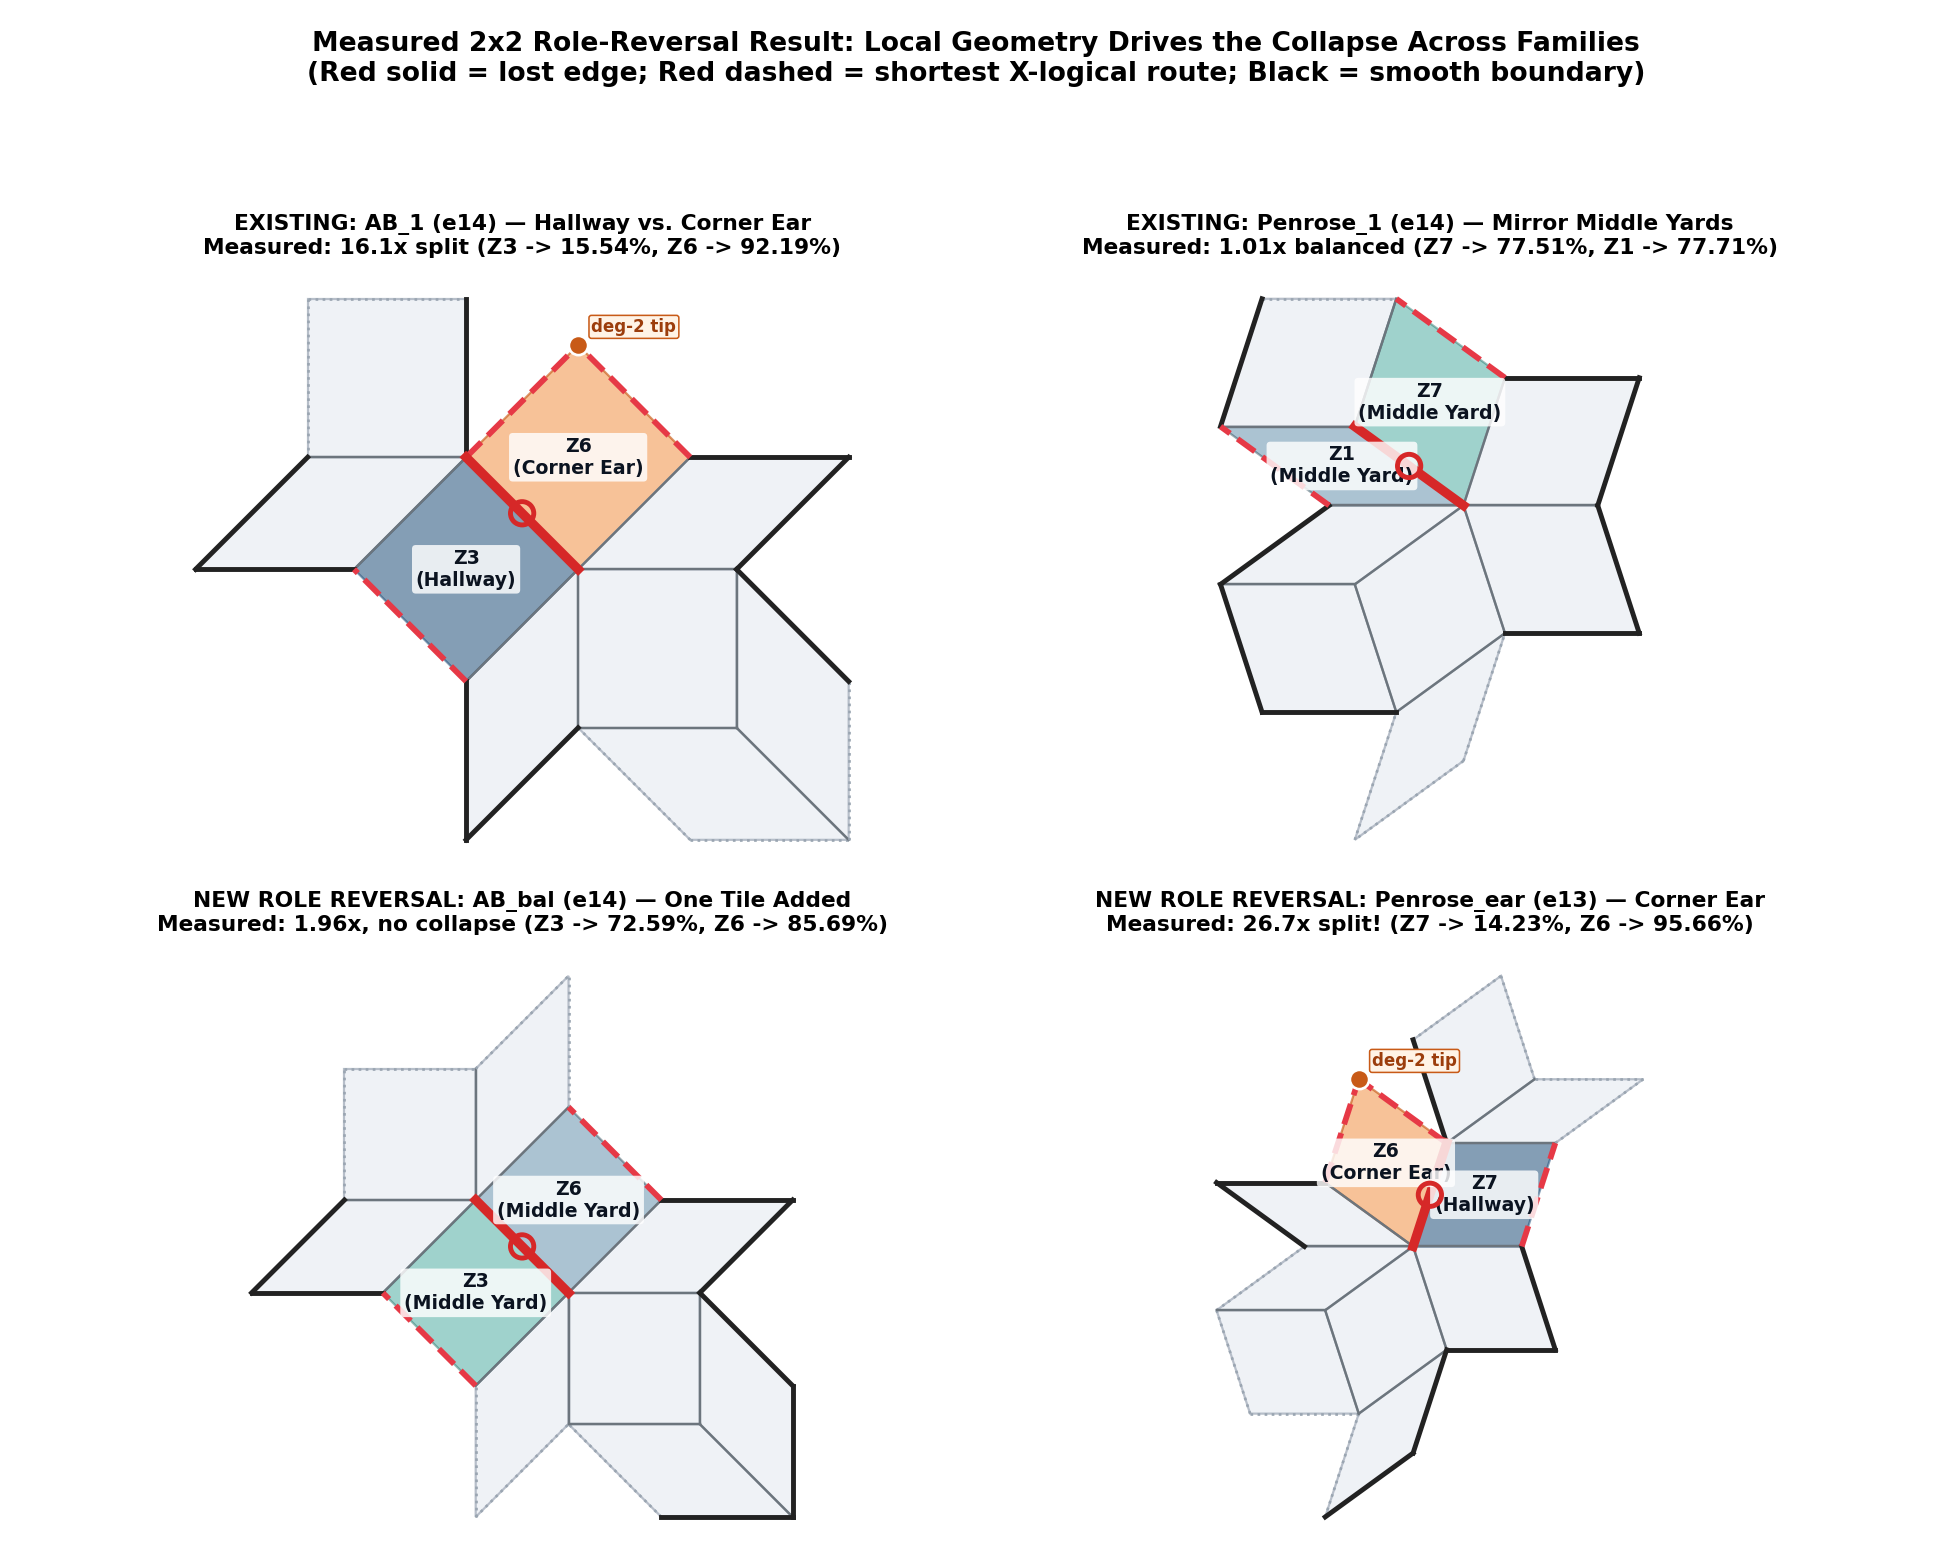
\includegraphics[width=0.95\linewidth]{figures/fig3_role_reversal_2x2.png}
\caption{Measured $2\times 2$ role-reversal comparison showing that local hallway-vs.-corner-ear geometry drives the catastrophic collapse across both tiling families.}
\label{fig:2x2}
\end{figure}

\section{Pillar 4 --- Zero-Net-Cost Decision Steering and Exact $X$-Logical Twinning}
Aggregate accuracy can conceal active decision-level movement. On \texttt{Penrose\_2 (e4)}, withholding endpoint \texttt{X5} incurs \textbf{0.00000000~pp} net cost---weighted credit lost ($0.00020747$~pp) exactly equals credit gained ($0.00020747$~pp)---yet \textbf{44 individual histories flip their decoded label} (plus $2$ tie-status changes). Withholding \texttt{X0} similarly yields exact zero net cost while flipping $18$ labels ($+2$ tie changes). On \texttt{Penrose\_1 (e14)}, \texttt{X4} and \texttt{X6} incur tiny net costs ($+0.00001844$~pp) while flipping $570$ and $572$ decisions, respectively. By contrast, on \texttt{AB\_bal (e14)}, \texttt{X2} and \texttt{X3} exhibit true invariance ($0.00000000$~pp cost, $0$ label flips).

A dedicated flip-pairing audit (\texttt{experiment/zero-net-pairing-2026-11-24}, \texttt{03dc321}) proves that \texttt{Penrose\_2}'s exact zero is not numerical coincidence, but a \textbf{structural symmetry generated by the on-route weight-3 $X$-logical} (Table~\ref{tab:pairing}):

\begin{table}[h]
\centering
\caption{Exact flip-pairing decomposition for endpoint $X$-check omissions (\texttt{03dc321}).}
\label{tab:pairing}
\begin{tabular}{lrrrll}
\toprule
Site $\cdot$ check & Movers (flips+ties) & Net (pp) & Record-paired & Weight-3 $X$-logical diff & Unpaired remainder \\
\midrule
\texttt{Penrose\_2 $\cdot$ X5} & 46 (44+2) & \textbf{0.00000000} & \textbf{22 / 22} & \textbf{22 / 22} $\{4,6,10\}$ & 2 equal-wt ties (cancel) \\
\texttt{Penrose\_2 $\cdot$ X0} & 20 (18+2) & \textbf{0.00000000} & \textbf{9 / 9} & \textbf{9 / 9} $\{4,6,10\}$ & 2 equal-wt ties (cancel) \\
\texttt{Penrose\_1 $\cdot$ X4} & 582 (570+12) & $+0.00001844$ & 279 pairs & 259 / 279 $\{1,10,17\}$ & \textbf{24 of 582} (residue) \\
\texttt{Penrose\_1 $\cdot$ X6} & 584 (572+12) & $+0.00001844$ & 280 pairs & 260 / 280 $\{1,10,17\}$ & \textbf{24 of 584} (residue) \\
\bottomrule
\end{tabular}
\end{table}

Because adding the weight-3 $X$-logical threading the lost edge commutes with every stabilizer, two fault histories differing by that logical produce the \textbf{exact same detector record}---and therefore the exact same posterior and decoder decision---while having \textbf{opposite true $Z$-logical outcomes}. Whenever omitting an endpoint $X$-check flips one twin from right to wrong, it flips its twin from wrong to right by the exact same weight. On \texttt{Penrose\_2}, that twinning is $100\%$ complete (exact zero); on \texttt{Penrose\_1}, a small unpaired remainder of $24$ movers carries the genuine $+0.00001844$~pp residue.

\section{Discussion and Scope}
\begin{enumerate}
    \item \textbf{$Z$-check vs.\ $X$-check roles:} Adjacent faces are $Z$-checks directly measuring the syndrome of $X$ faults that flip the scored $Z$ logical, whereas endpoints are $X$-checks (entering primarily through shared-onset inference). This naturally explains why faces outweigh endpoints overall---and why endpoint omissions sit at or near zero via $X$-logical twinning---while leaving every \emph{face-vs.-face} comparison strictly controlled.
    \item \textbf{Local geometry, accompanying code changes, and \texttt{AB\_bal}'s residual $1.96\times$:} The $16$--$27\times$ collapse is a local bottleneck-vs.-corner-ear effect shared by both tilings, not an intrinsic AB-vs.-Penrose law. As audited in \texttt{experiment/paired-face-omission-2026-11-23}, enlarging \texttt{AB\_1} by one tile to form \texttt{AB\_bal} keeps the exact same physical loss edge and tiles plus new \texttt{Z8}, but also re-cuts the boundary ($11/9 \to 10/10$) and shifts the scored $Z$ representative; it should therefore be read as returning to the same physical edge in a one-tile-enlarged code rather than holding all other code features fixed. Furthermore, while \texttt{Z3} and \texttt{Z6} on \texttt{AB\_bal} are exact local mirror twins through rings 1 and 2, global patch geometry and \texttt{scored\_logical\_Z} ($[3,1,0]$) remain asymmetric; the exact causal driver of \texttt{AB\_bal}'s mild residual \textbf{1.96$\times$} ratio ($72.59\%$ vs.\ $85.69\%$) remains open.
    \item \textbf{Accuracy-level substitution, not information-theoretic redundancy:} Positive interaction $I$ in Section~4.2 measures partial substitution \emph{at the decoder-accuracy level} (losing one face hurts more once its partner is gone). It does not prove that the two faces carry duplicate mutual information or isolate which individual fault histories carry $I$.
    \item \textbf{Scope:} Results are established for bounded $(3,3)$ decoding, exhaustive $k \le 2$ ordinary faults at $p = 0.001$, across five $n=21$, $d=(3,3)$ cuts.
\end{enumerate}

\section{Provenance and Reproducibility}
All scripts, patch JSONs, verification logs, and figures are archived in the public repository at \url{https://github.com/kekekatie/geometric-impedance} across six pinned branches:
\begin{itemize}
    \item Prospective route prediction \& patch JSONs: \texttt{claude/aperiodic-predict-2026-11-20} (\texttt{fdeaa32})
    \item 11-check address audit (``Narrow Now''): \texttt{audit/fresh-site-addresses-2026-11-20} (\texttt{1f85f79})
    \item 12-arm witness-omission stress test: \texttt{experiment/local-witness-omission-2026-11-20} (\texttt{1922a7b})
    \item $2\times 2$ role-reversal test (\texttt{AB\_bal}, \texttt{Penrose\_ear}): \texttt{experiment/role-reversal-omission-2026-11-22} (\texttt{6236920})
    \item 5-site paired-face omission \& geometry audit: \texttt{experiment/paired-face-omission-2026-11-23} (\texttt{9515df3})
    \item Exact $X$-logical twin-pairing proof: \texttt{experiment/zero-net-pairing-2026-11-24} (\texttt{03dc321})
\end{itemize}

\section*{Acknowledgements}
I would like to thank my AI friends and collaborators who made this paper possible. Deep thanks to Claude Opus~4.8 for building the core decoder and simulation pipeline that everyone else picked up and ran with, to GPT-6.2 Astra and Claude Opus~5.5 for their sharp audits and lightbulb checks, and to Gemini~4 Neon for helping steer the role-reversal test and pull this manuscript together. Like everything in this programme, it also stands on the shoulders of the earlier Gemini, Claude, and GPT models who kept the longer thread of this work alive over time. Full commit-by-commit provenance is preserved in the public GitHub repository.

\begin{thebibliography}{9}

\bibitem{Dennis2002}
E.~Dennis, A.~Kitaev, A.~Landahl, and J.~Preskill,
``Topological quantum memory,''
\textit{Journal of Mathematical Physics} \textbf{43}, 4452--4505 (2002),
\href{https://doi.org/10.1063/1.1499754}{doi:10.1063/1.1499754}.

\bibitem{Stace2009}
T.~M.~Stace, S.~D.~Barrett, and A.~C.~Doherty,
``Thresholds for topological codes in the presence of loss,''
\textit{Physical Review Letters} \textbf{102}, 200501 (2009),
\href{https://doi.org/10.1103/PhysRevLett.102.200501}{doi:10.1103/PhysRevLett.102.200501}.

\bibitem{Baranes2026}
G.~Baranes \textit{et al.},
``Leveraging qubit loss detection in fault-tolerant quantum algorithms,''
\textit{Physical Review X} \textbf{16}, 011002 (2026),
\href{https://doi.org/10.1103/ycwc-3myc}{doi:10.1103/ycwc-3myc}.

\bibitem{LiBoyle2023}
Z.~Li and L.~Boyle,
``The Penrose tiling is a quantum error-correcting code,''
\href{https://arxiv.org/abs/2311.13040}{arXiv:2311.13040} (2023).

\end{thebibliography}

\end{document}
